\documentclass[tikz]{standalone}

\definecolor{n0}{HTML}{785EF0}
\definecolor{End}{HTML}{DC267F}
\definecolor{Corner}{HTML}{FFB000}
\definecolor{Reversal}{HTML}{FE6100}

\begin{document}
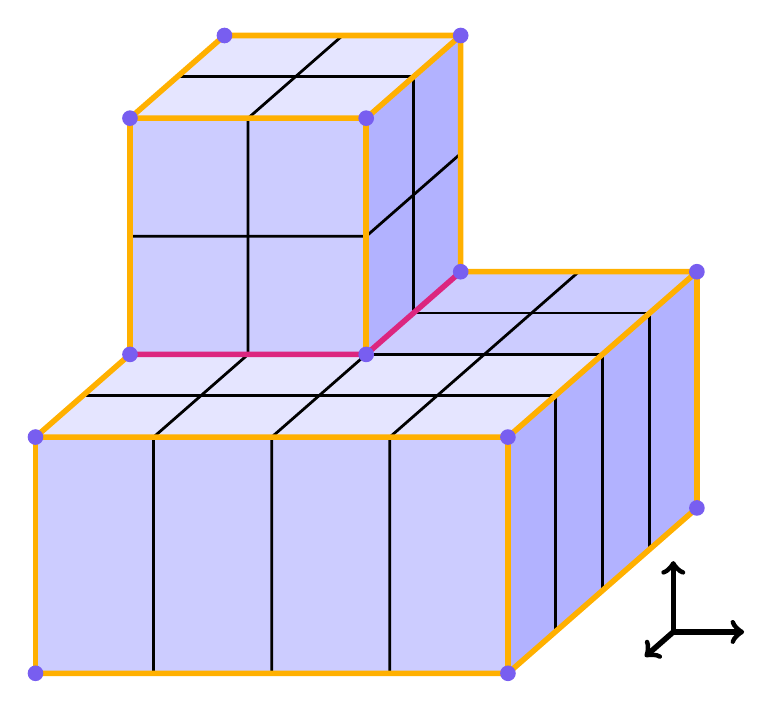
\begin{tikzpicture}[scale=3, x={(1cm,0cm)}, y={(0cm,1cm)}, z={(-0.4cm,-0.35cm)}]

  %%%%%%%%%%%%%%%% AXES %%%%%%%%%%%%%%%%%%%%%%
  \draw [->, line width=2] (1.5,-1,0.5) -- (1.8,-1,0.5) ;
  \draw [->, line width=2] (1.5,-1,0.5) -- (1.5,-0.7,0.5) ;
  \draw [->, line width=2] (1.5,-1,0.5) -- (1.5,-1,0.8) ;

 %%%%%%%%%% Points pour travailler %%%%%%%%%%
 \coordinate (0) at (-1,-1,1);
 \coordinate (1) at (0,-1,1);
 \coordinate (2) at (1,-1,1);
 \coordinate (3) at (-1,0,1);
 \coordinate (4) at (0,0,1);
 \coordinate (5) at (1,0,1);
 \coordinate (6) at (-1,-1,0);
 \coordinate (7) at (0,-1,0);
 \coordinate (8) at (1,-1,0);
 \coordinate (9) at (-1,0,0);
 \coordinate (10) at (0,0,0);
 \coordinate (11) at (1,0,0);
 \coordinate (12) at (-1,1,0);
 \coordinate (13) at (0,1,0);
 \coordinate (14) at (-1,-1,-1);
 \coordinate (15) at (0,-1,-1);
 \coordinate (16) at (1,-1,-1);
 \coordinate (17) at (-1,0,-1);
 \coordinate (18) at (0,0,-1);
 \coordinate (19) at (1,0,-1);
 \coordinate (20) at (-1,1,-1);
 \coordinate (21) at (0,1,-1);
 
 % Surface Mesh
 \draw [line width=1, fill=blue!20!white] (0) -- (2) -- (5) -- (3) -- (0) ;
 \draw [line width=1, fill=blue!20!white] (18) -- (19) -- (5) -- (4) -- (18) ;
 \draw [line width=1, fill=blue!10!white] (3) -- (5) -- (11) -- (9) -- (3) ;
 \draw [line width=1, fill=blue!30!white] (2) -- (5) -- (19) -- (16) -- (2) ;
 

 \draw [line width=1, fill=blue!20!white] (9) -- (10) -- (13) -- (12) -- (9) ;
 \draw [line width=1, fill=blue!10!white] (12) -- (13) -- (21) -- (20) -- (12) ;
 \draw [line width=1, fill=blue!30!white] (10) -- (18) -- (21) -- (13) -- (10) ;


 \draw [line width=1] (1) -- (4) -- (10);
 \draw [line width=1] (11) -- (8);


 %%%%%%%%%%%%%% REFINED MESH %%%%%%%%%%%%%%
 \coordinate (30) at (-0.5,-1,1);
 \coordinate (31) at (0.5,-1,1);
 \coordinate (32) at (-1,-1,0.5);
 \coordinate (33) at (-0.5,-1,0.5);
 \coordinate (34) at (0,-1,0.5);
 \coordinate (35) at (0.5,-1,0.5);
 \coordinate (36) at (1,-1,0.5);
 \coordinate (37) at (-0.5,-1,0);
 \coordinate (38) at (0.5,-1,0);
 \coordinate (39) at (-1,-1,-0.5);
 \coordinate (40) at (-0.5,-1,-0.5);
 \coordinate (41) at (0,-1,-0.5);
 \coordinate (42) at (0.5,-1,-0.5);
 \coordinate (43) at (1,-1,-0.5);
 \coordinate (44) at (-0.5,-1,-1);
 \coordinate (45) at (0.5,-1,-1);
 \coordinate (46) at (-0.5,0,1);
 \coordinate (47) at (0.5,0,1);
 \coordinate (48) at (-1,0,0.5);
 \coordinate (49) at (-0.5,0,0.5);
 \coordinate (50) at (0,0,0.5);
 \coordinate (51) at (0.5,0,0.5);
 \coordinate (52) at (1,0,0.5);
 \coordinate (53) at (-0.5,0,0);
 \coordinate (54) at (0.5,0,0);
 \coordinate (55) at (-1,0,-0.5);
 \coordinate (56) at (0,0,-0.5);
 \coordinate (57) at (0.5,0,-0.5);
 \coordinate (58) at (1,0,-0.5);
 \coordinate (59) at (-0.5,0,-1);
 \coordinate (60) at (0.5,0,-1);
 \coordinate (61) at (-1,0.5,0);
 \coordinate (62) at (-0.5,0.5,0);
 \coordinate (63) at (0,0.5,0);
 \coordinate (64) at (-1,0.5,-0.5);
 \coordinate (65) at (0,0.5,-0.5);
 \coordinate (66) at (-1,0.5,-1);
 \coordinate (67) at (-0.5,0.5,-1);
 \coordinate (68) at (0,0.5,-1);
 \coordinate (69) at (-0.5,1,0);
 \coordinate (70) at (-1,1,-0.5);
 \coordinate (71) at (-0.5,1,-0.5);
 \coordinate (72) at (0,1,-0.5);
 \coordinate (73) at (-0.5,1,-1);


 %%%%% New edges %%%%%
 \draw [line width=1] (30) -- (46) -- (53) -- (69) -- (73) ;
 \draw [line width=1] (60) -- (47) -- (31) ;
 \draw [line width=1] (70) -- (72) -- (56) -- (58) -- (43) ;
 \draw [line width=1] (48) -- (52) -- (36) ;
 \draw [line width=1] (61) -- (63) -- (68) ;


  % Corner Edges
 \draw[line width=2, color=Corner] (0) -- (2);
 \draw[line width=2, color=Corner] (0) -- (2) -- (16);
 \draw[line width=2, color=Corner] (0) -- (3);
 \draw[line width=2, color=Corner] (2) -- (5);
 \draw[line width=2, color=Corner] (16) -- (19);
 \draw[line width=2, color=Corner] (20) -- (12) -- (9) -- (3) -- (5) -- (19) -- (18) -- (21) -- (20);
 \draw[line width=2, color=Corner] (12) -- (13) -- (21);
 \draw[line width=2, color=Corner] (9) -- (12);
 \draw[line width=2, color=Corner] (10) -- (13);
 \draw[line width=2, color=Corner] (18) -- (21);

 % End Edges
 \draw[line width=2, color=End] (9) -- (10) -- (18);

 % Feature Nodes
 \draw (0) node[circle, fill=n0, inner sep = 2pt] {};
 \draw (2) node[circle, fill=n0, inner sep = 2pt] {};
 \draw (3) node[circle, fill=n0, inner sep = 2pt] {};
 \draw (5) node[circle, fill=n0, inner sep = 2pt] {};
 \draw (9) node[circle, fill=n0, inner sep = 2pt] {};
 \draw (10) node[circle, fill=n0, inner sep = 2pt] {};
 \draw (12) node[circle, fill=n0, inner sep = 2pt] {};
 \draw (13) node[circle, fill=n0, inner sep = 2pt] {};
 \draw (16) node[circle, fill=n0, inner sep = 2pt] {};
 \draw (18) node[circle, fill=n0, inner sep = 2pt] {};
 \draw (19) node[circle, fill=n0, inner sep = 2pt] {};
 \draw (20) node[circle, fill=n0, inner sep = 2pt] {};
 \draw (21) node[circle, fill=n0, inner sep = 2pt] {};

\end{tikzpicture}
\end{document}